\chapter{The Daya Bay Experiment}

\section{The Daya Bay Site}
To measure $\theta_{13}$, an experimental site with high thermal power of reactors to supply large antineutrino flux and with mountains nearby to serve as cosmic ray shielding is required. Daya Bay is the appropriate site meeting the requirements.

The Daya Bay reactor complex is located on the southeast coast of China, 55 km northeast of Hong Kong. The reactor complex is composed of 3 nuclear power plants, namely the Daya Bay (DYB) nuclear power plant, the Ling Ao (LA) nuclear power plant and the Ling Ao-II (LA II) nuclear power plant. Each nuclear power plant is equipped with a pair of functionally identical pressurized water reactors (PWR) separated by 90 m. Each reactor core supplies 2.9 GW thermal power. The Ling Ao nuclear power plant is \textasciitilde 1100 m from the Daya Bay nuclear power plant, and the Ling Ao-II is \textasciitilde 500 m from the Ling Ao. On the other hand, the Daya Bay experimental facility is composed of 3 underground experimental halls, a surface assembly building, a liquid scintillator (LS) hall and a water hall (EH4). The underground halls are connected by horizontal tunnels. The 3 experimental halls are where the antineutrino detectors and the muon detectors are installed. The experimental hall closest to the Daya Bay/Ling Ao nuclear power plant is called the Daya Bay/Ling Ao near site, or experimental hall 1/2 (EH1/EH2). The experimental hall farthest from all the reactor cores is called the Far site, or experimental hall 3 (EH3). The surface assembly building is the place where people assemble the antineutrino detector (AD), do the dry run test and other detector related work before transporting equipment underground. The LS hall is where Daya Bay's liquid scintillator and Gd-doped liquid scintillator are produced and the ADs are filled. The water hall is where the ultra purity water system is placed which supplies ultra purity water to the 3 water pools in EH1, EH2 and EH3. Figure~\ref{fig:dybsite} shows experimental facility and the 6 reactor cores. The distances from the centroids of each reactor pair to the sites is shown in Table~\ref{tab:sitecoredist}.

\begin{figure}
	\centering
	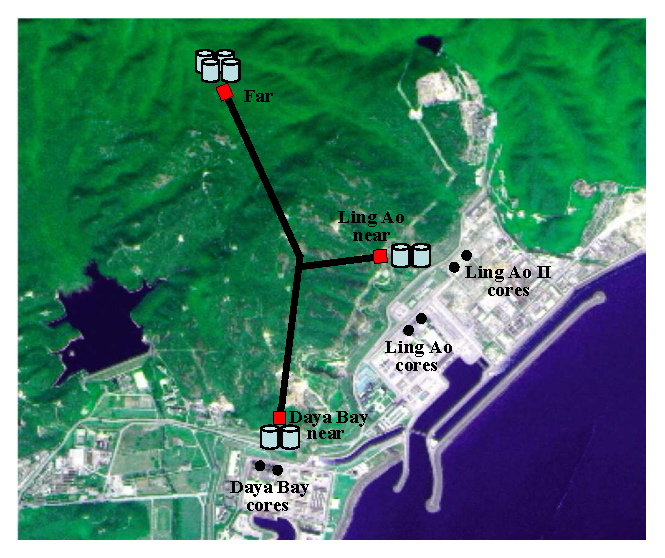
\includegraphics[width=0.45\textwidth]{figures/chap2/dayabay_site.eps}
	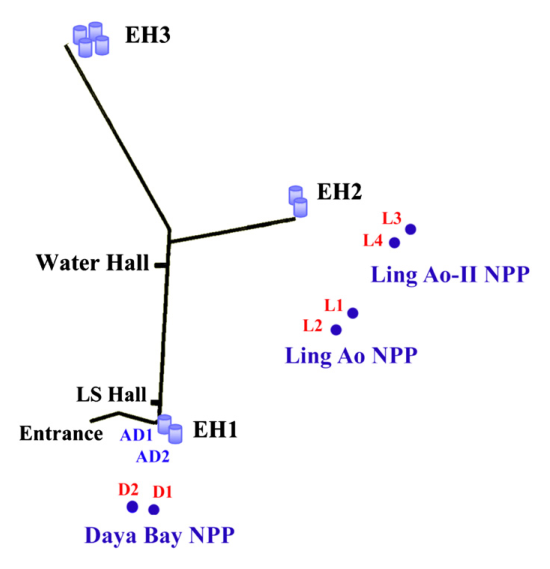
\includegraphics[width=0.35\textwidth]{figures/chap2/dayabay_site_illustration.eps}
	\caption{The Daya Bay site.}
	\label{fig:dybsite}
\end{figure}

\begin{table}
	\centering
	\begin{tabular}{|c|c|c|c|}
	\hline
	& DYB & LA & FAR \\
	\hline
	DYB cores & 363 & 1347 & 1985 \\
	\hline
	LA cores & 857 & 481 & 1618 \\
	\hline
	LA II cores & 1307 & 526 & 1613 \\
	\hline
	\end{tabular}
	\caption{Distances from the centroids of each reactor pair to the sites.}
	\label{tab:sitecoredist}
\end{table}


\section{The Antineutrino Detector}

The antineutrino detectors(ADs) are the main detectors used for detecting neutrinos via the inverse beta decay reaction. Figure~\ref{fig:CSAD} shows the cross sectional view of the design of the Daya Bay AD. The AD is separated into 3 different zones by 3 coaxial cylindrical vessels. They are the stainless steel vessel (SSV), the outer acrylic vessel (OAV) and the inner acrylic vessel (IAV) from the outside in. The SSV is a 5 m high cylinder with a 5 m diameter. The OAV is a 4 m high cylinder with a 4 m diameter while the IAV is a 3 m high cylinder with a 3 m diameter. Inside the IAV is the neutrino target filled with 20 t liquid scintillator doped with gadolinium whose concentration is $0.1\%$ by weight. 21 t of unloaded liquid scintillator (LS) is filled between the IAV and the OAV which serves as the $\gamma$ catcher. The outermost region between the IAV and the SSV is filled with 37 t of mineral oil and is call the buffer layer.
\begin{figure}
	\centering
	\includegraphics[width=0.7\textwidth]{figures/chap2/AD_cross_section.eps}
	\caption{Cross sectional view of the Daya Bay antineutrino detector.}
	\label{fig:CSAD}
\end{figure}
Each antineutrino detector is equipped with 192 8-inch Hamamatsu R5912 PMTs mounted on 8 ladders along the circumference of the SSV and within the mineral oil region.

\subsection{The Liquid Scintillator}
The liquid scintillator is 


\section{The Muon System}

To shield the ADs from backgrounds introduced by cosmic ray muons, the ADs are surrounded by muon detectors. The muon system consists of two detector subsystems. One is the water pool in which ADs are submerged which serves as a water Cerenkov counter. The other is the Resistive Plate Chamber(RPC) system which covers the water pool.

\subsection{The Water Cerenkov Detector}

When a charged particle passes through a medium at a speed faster than the speed of light in the medium, Cerenkov radiation will be generated. If PMTs are mounted inside the detector facing the medium, charged particles can be detected by the Cerenkov detector with high efficiency by counting the number of PMTs receiving Cerenkov photons.



\subsection{The Resistive Plate Chambers}

In addition to the water pool itself, the water pool is covered by another muon detector called resistive plate chamber(RPC). The RPCs are basically parallel plate gas detectors whose detailed physics will be discussed in the next chapter. This design of muon system not only increases the muon tagging efficiency but also greatly increases the accuracy of the muon track reconstruction.



\section{The Electronics, Data Acquisition and Offline Software}

For the ADs, each AD PMT raw signals are connected to the Front End Electronics boards (FEEs). Every FEE board has up to 16 channels and can do a charge integration and count for the number of PMT channels over the threshold. The system trigger can be issued by the total energy or total number of fired PMTs.

Daya Bay's offline software, NuWa, is a software framework based on Gaudi which is developed at LHCb. By definition a software framework is software which provides generic functionality and in which users can add additional user's own codes to do specific jobs.